\fullwidth{Use the following figure to answer the next three questions.}

\vspace*{-0.5\baselineskip}
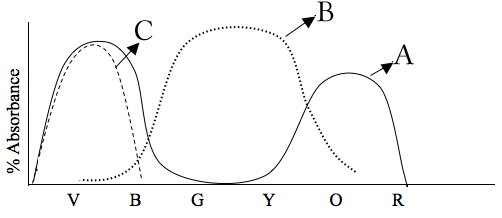
\includegraphics[width=0.5\textwidth]{absorbanceA}


\question
Line A represents the absorption spectrum of which group of photopigments? 
\ifprintanswers{\textbf{carotenoids}}\fi\vspace*{1\baselineskip}

\question
Line B represents the absorption spectrum of which group of photopigments?
\ifprintanswers{\textbf{chlorophyll}}\fi\vspace*{1\baselineskip}

\question
Line C represents the absorption spectrum of which group of photopigments?
\ifprintanswers{\textbf{phycobilins}}\fi\vspace*{1\baselineskip}

\question[4]
Write a \emph{balanced} chemical equation for photosynthesis.  
\ifprintanswers{\ce{6CO2 + 6H2O -> C6H12O6 + 6O2 + 6 H2O}}\\
{\bfseries Subtract 1 pt if one prefix number is missing or wrong (e.g., \ce{4H2O}, 2 pts if more than 1 is wrong. \\
Subtract 1 pt if one chemical formula is wrong (e.g., \ce{C12H6O6}), 2 pts if one missing more more than 1 wrong.\\Ask me if uncertain.}
\fi 
\vspace*{2\baselineskip}
